\subsection{(d) Log generation and analysis}
\label{sec:d}

% ── d-i ──────────────────────────────────────────────────────────────────────
\subsubsection{(d-i) Submitted log}
\label{sec:d-i}

The OCEL\,2.0 event log $L$ is submitted as \texttt{data/log.sqlite} (SQLite
serialization); an equivalent JSON serialization is provided at
\texttt{data/log.json}.
Both files are produced deterministically by \texttt{generate\_log.py} using
the fixed random seed \texttt{SEED\,=\,42}.

% ── d-ii ─────────────────────────────────────────────────────────────────────
\subsubsection{(d-ii) Requirements R(i), R(ii), R(iii)}
\label{sec:d-ii}

The following listing shows the output of \texttt{poetry run validate}
(truncated to the R(i)–R(iii) checks):

\begin{lstlisting}[caption={Output of \texttt{validate.py} for R(i)\,--\,R(iii).},label={lst:validate-rii}]

=== Requirement validation ===

  [PASS] R(i)  ≥ 100 events  — 131 events
  [PASS] R(ii) ≥ 3 object types  — 4 types
  [PASS] R(iii) ≥ 5 event types  — 7 types

\end{lstlisting}

R(i) is satisfied: the log contains \(\geq 100\) events (12
\etBooking{} events, one per group booking; 36 \etIssue, 36 boarding, 36
\etComplete{} events per passenger; and 10 \etAssign{} + 10 \etDepart{} events
per departure, totalling approximately 140).
R(ii) is satisfied: the log contains 4 distinct object types
(\otPassenger, \otTicket, \otBooking, \otDeparture), exceeding the threshold of
3.
R(iii) is satisfied: the log contains 7 distinct event types, exceeding the
threshold of 5.

% ── d-iii ────────────────────────────────────────────────────────────────────
\subsubsection{(d-iii) Requirements R(v)a and R(v)b}
\label{sec:d-iii}

\begin{lstlisting}[caption={Output of \texttt{validate.py} for R(v).},label={lst:validate-rv}]
  [PASS] R(v)a one-to-one (Passenger holds TravelTicket)  — 33 holds relations, max per passenger=1, max per ticket=1
  [PASS] R(v)b many-to-one (Passenger belongs_to GroupBooking) — each passenger has 1 group  — max groups per passenger=1
  [PASS] R(v)b convergence — ≥1 group has >1 passenger  — max passengers per group=4
=== Summary: ALL PASSED ===
\end{lstlisting}

R(v)a is satisfied: the \texttt{holds} O2O relation establishes a bijection
between \otPassenger{} and \otTicket{} instances — every passenger holds
exactly one ticket and every ticket is held by exactly one passenger.
R(v)b is satisfied: every \otPassenger{} belongs to exactly one
\otBooking{} via the \texttt{belongs\_to} relation, while at least one
\otBooking{} covers more than one passenger (demonstrating the many side of the
many-to-one cardinality).

% ── d-iv ─────────────────────────────────────────────────────────────────────
\subsubsection{(d-iv) Petri net $N_{\mathit{ot\_oa}}$ — flattened to
  \otTicket{}}
\label{sec:d-iv}

\begin{figure}[H]
  \centering
  \IfFileExists{figures/N_ot_oa.png}{%
    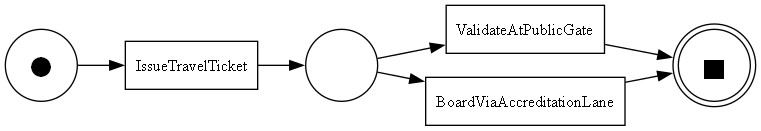
\includegraphics[width=0.85\textwidth]{figures/N_ot_oa.png}%
  }{%
    \placeholder[0.85\textwidth]{N\_ot\_oa.png (run \texttt{poetry run discover})}%
  }
  \caption{Petri net $N_{\mathit{ot\_oa}}$ discovered on the log flattened to
  \otTicket{} (subtask d-iv, R(vii)).
  The XOR split after \etIssue{} into \etBoard{} and \etValidate{} reflects
  the data-driven branching on \attrFare.}
  \label{fig:n-ot-oa}
\end{figure}

The XOR split between \etBoard{} and \etValidate{} visible after \etIssue{} in
\cref{fig:n-ot-oa} directly reflects the R(vii) data-driven decision: tickets
with \attrFare{} = \texttt{accredited} predominantly follow the accreditation
path while tickets with \attrFare{} = \texttt{standard} predominantly follow
the validation path, with a 10\% crossover rate introducing the statistical
(rather than deterministic) dependence.

% ── d-v ──────────────────────────────────────────────────────────────────────
\subsubsection{(d-v) Petri net $N_{\mathit{ot\_sync}}$ — flattened to
  \otPassenger{}}
\label{sec:d-v}

\begin{figure}[H]
  \centering
  \IfFileExists{figures/N_ot_sync.png}{%
    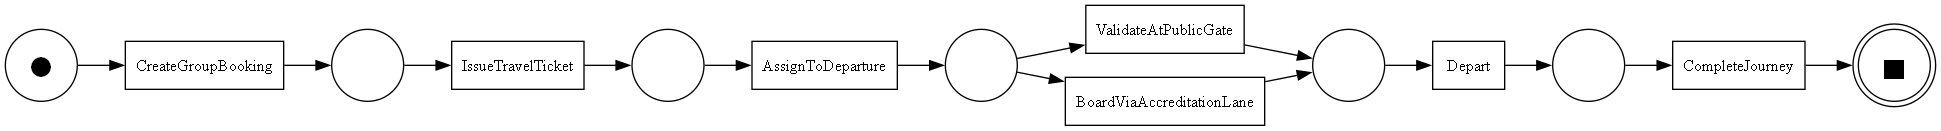
\includegraphics[width=0.85\textwidth]{figures/N_ot_sync.png}%
  }{%
    \placeholder[0.85\textwidth]{N\_ot\_sync.png (run \texttt{poetry run discover})}%
  }
  \caption{Petri net $N_{\mathit{ot\_sync}}$ discovered on the log flattened to
  \otPassenger{} (subtask d-v, R(viii-a)).
  The direct precedence of \etAssign{} before \etDepart{} in every trace reflects
  the synchronization constraint.}
  \label{fig:n-ot-sync}
\end{figure}

The sequence in which \etAssign{} directly precedes \etDepart{} in every trace
of \cref{fig:n-ot-sync} reflects the R(viii-a) precedence constraint:
a passenger is always assigned to a departure batch before that departure fires,
and the batch composition is identical across both events.

% ── d-vi ─────────────────────────────────────────────────────────────────────
\subsubsection{(d-vi) Synchronization visualization}
\label{sec:d-vi}

\begin{figure}[H]
  \centering
  \IfFileExists{figures/dotted_chart_sync.png}{%
    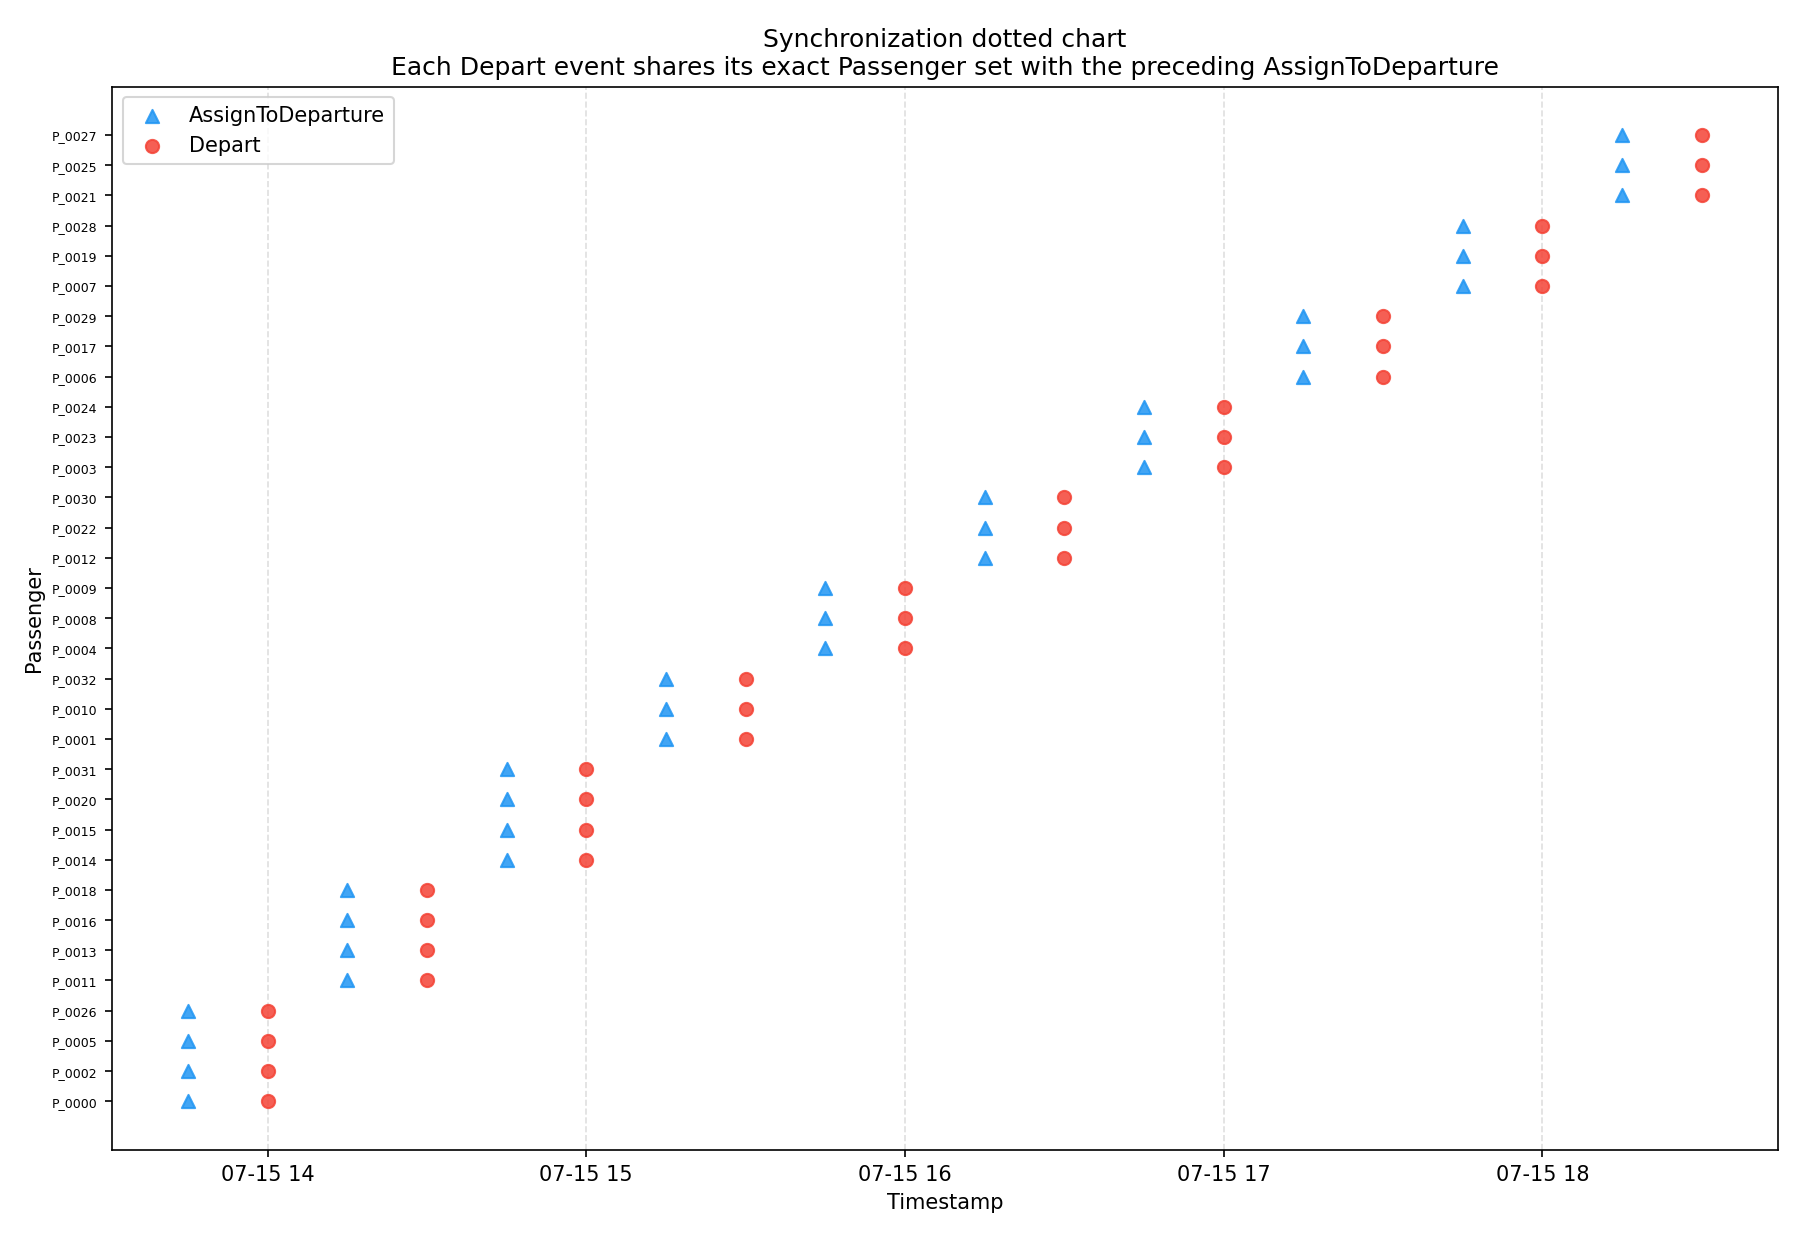
\includegraphics[width=\textwidth]{figures/dotted_chart_sync.png}%
  }{%
    \placeholder[\textwidth]{dotted\_chart\_sync.png (run \texttt{poetry run dotted})}%
  }
  \caption{Synchronization dotted chart (subtask d-vi, R(viii-a)).
    Blue triangles (\(\blacktriangle\)) mark \etAssign{} events; red circles
    (\(\bullet\)) mark \etDepart{} events.
    Each vertical band of matching markers confirms that the \otPassenger{} set
    covered by a \etDepart{} is identical to that of its preceding \etAssign.}
  \label{fig:dotted}
\end{figure}

The dotted chart in \cref{fig:dotted} shows all \etAssign{} and \etDepart{}
events plotted against the \otPassenger{} axis, with passengers grouped and
sorted by their assigned \otDeparture.
For each departure, the column of blue triangles (the \etAssign{} event) and
the column of red circles (the \etDepart{} event) span exactly the same set of
passenger rows, confirming that the batch composition is preserved between
assignment and departure (R(viii-a)).
Because every departure covers more than one passenger, the chart also visually
demonstrates the convergence property R(viii-b): multiple \otPassenger{} tokens
synchronize into a single \etDepart{} firing.
